\documentclass[11pt]{article}
\usepackage{graphicx}

\begin{document}
	
	
	{\centering {\Large SEBASTIAN PORRAS GARULO\\
	 
	 Asignment 2\\ \par}}

	
	\textbf {Excercise 1\\}
	
	A) 	The expected value of the prospect is $EV=0.2\cdot 40+0.6\cdot 50+0.2\cdot 30=44$ and the utility given the formula  $U(x)= \sum_{i} p_i u_i$ is $0.2\cdot 40/10 + 0.6\cdot  50/10 + 0.2\cdot  30/10 = 4.4$.\\
	The certainty equivalent (CE) is calculated by determining the value of x for which an individual is indifferent of receiving the prospect or a certain amount. In this case, since utility is given by $U(x)= x/10$, the CE is calculated as follows:
	
	\[U(x)=4.4\]
	\[4.7=  x/10\]
	\[x= 4.4\cdot 10=44=CE\]
	
	B) 	The rank dependent utility calculated using $U(x)= \sum_{i} \pi_{i} \cdot u_{i}$ and $w(p)= p^2$ is as follows: $0.2^2 \cdot 4+(0.8^2-0.2^2)\cdot 5+(1^2-0.8^2)\cdot 3=4.24$.\\
	Given that the utility is calculated as u(x)=0.1*x , so the amount for which an individual would be indifferent between the prospect or a certain amount would be $4.24/0.1=42.4=CE$.\\
	
	
	\textbf {Excercise 2\\}
	
	Under the expected utility theory, prospect E and prospect F yield the same outcome (750). Prospect G and prospect H both yield an expected utility of 1500. Levy and Levy (2002) reject the S-shaped utility function of the Cumulative Prospect Theory (CPT) because they found a preference for E (71\% of the subjects) and a preference for G (76\% of the subjects. Under CPT, the S-shaped utility function is concave for gains and convex for losses, meaning that individuals are risk-averse for gains and risk-seeking for losses. Applied to the prospects illustrated in the question, since the expected utility is the same, individuals should choose prospects F and H. So, in line with the research of Levy and Levy (2002), we also reject the S-shaped curve based on the results of L\&L. However, L\&L don’t account for the probability weighting function as Kahneman and Tversky (1992) did. They state in their paper: “All probabilities given in the experiments are relatively large $(p ≥ 0.25)$, hence it is unlikely that subjective probability distortion plays an important role in the decision-making process”. When probability weighting is considered (Wakker, P., 2003), the optimal choices shift from E to F and from G to H, implying that the conclusion of L\&L is unfounded. \\
		
		\begin{figure}[ht] 
		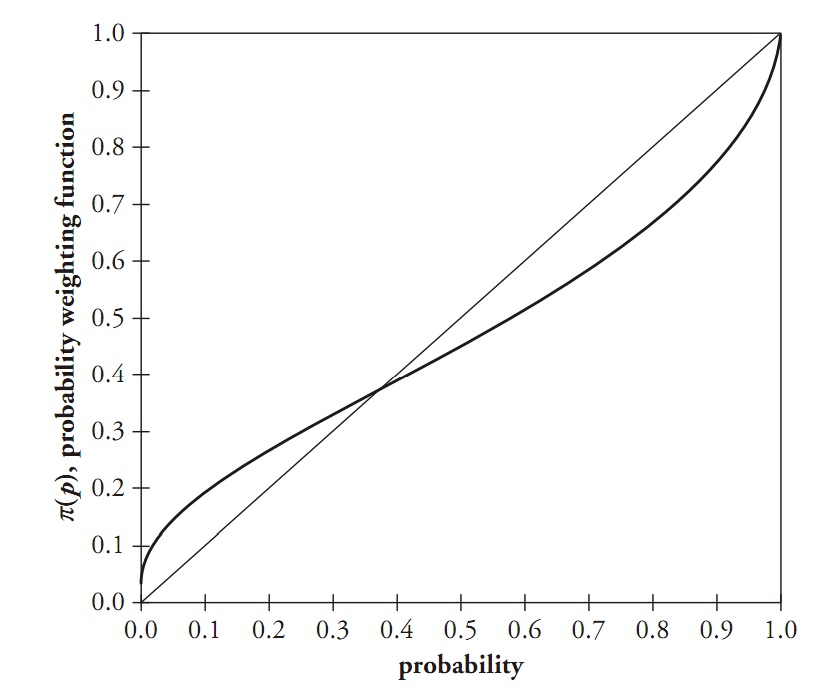
\includegraphics{WeightedProbability.jpg}
		\caption{As we can see, the low probability is weighted highly, while the tall probabilities are weighted lowly.}
		\end{figure}
	

	
	The conclusion of Levy and Levy would have been correct if they had taken into account the probability weighting, but because this wasn’t the case, we do not agree with the conclusion that the S-shaped utility curve is rejected.
	


\end{document}